\documentclass[12pt]{article}

% Geometry
\usepackage[a4paper, left=3cm, right=2.5cm, top=2.5cm, bottom=3cm]{geometry}

% Font encoding
\usepackage[utf8]{inputenc} % UTF-8 encoding
\usepackage[T1]{fontenc} % Font encoding
\usepackage{times}

% Math packages
\usepackage{amsmath} % Basic math symbols and environments
\usepackage{amssymb} % Additional math symbols
\usepackage{amsfonts} % Math fonts

% Pictures
\usepackage{graphicx}

% Lists
\usepackage{enumitem}
\setlist[itemize]{topsep=-0.5em}

% Bibliography
%\usepackage{cite}

% Title and author
\title{Econometrics I - Empirical Work}
\author{Ricardo Semião e Castro}
\date{04/2024}


\begin{document}

\maketitle

\section{Introduction}

Before going to the questions, I'll present some topics on the empirical strategy that are relevant to the whole exercise.a

The empirical papers in the literature often do some kind of filtering of the data. There are a lot of different types of households and families, there is a important trade-off in cleaning "bad" cases, such as families with absent parents, step children, old "children", etc. On one hand, filtering removes noise and biases, helping the interpretation of the results; but, on the other (i) we lose observations, which yield less precise inference, (ii) reduces the population being studied and the extrapolation potential, and (iii), if poorly made, might induce a selection bias and/or be seen as arbitrary.

In the present case, the selected census, of Puerto Rico 2000, had $13,372$ households, with only $6,512$ with children, such that item (i) is really relevant, some "bad" cases were too costly to remove. Below I present the filtering strategy used in this exercise:

\begin{itemize}
    \item Households without children were removed.
    \begin{itemize}
        \item Defining children as descendants under 18 years old (the ``medium'' legal age in Puerto Rico), there are $25.48\%$ of original households with children. This is a very low sample size, so it was considered children as descendants under 21 years old (the full legal age in Puerto Rico), but that aren't yet married nor working, such that they're probably still accounted by the parents in the development decision. We're left with $28.21\%$ of original cases, $3,970$ households. The percentages below refer to this baseline.
    \end{itemize}
    \item Households with more than one family were removed ($1.66\%$ of cases), as it is hard to argue how is the development decision made, at the family or at the household level;
    \item Households classified as "group quarters" were removed ($0.1\%$ of cases), for the same reason as above;
    \item Households with absent mothers were removed ($3.33\%$ of cases).
    \begin{itemize}
        \item Absent fathers were a lot more common ($33.4\%$ of the cases), and had to be kept. The literature seems to give more focus on the mother's role in the child's development, such that keeping households with absent fathers is less problematic. I also discuss including a control for this;
        \item Households with step parenting were kept ($7.54\%$ of the cases) as it was assumed that different parenting status didn't changed too much the development decision. I also discuss including a control for this;
    \end{itemize}
    \item Households where there were descendants of the head of the family with more than 21 years old were removed, even tough they had a large presence ($12.53\%$ of original cases). In these households, the old descendants enter completely differently in the development decision, such that a lot of noise comes from these cases.
    \item Households where there were simultaneously children and grandchildren were removed ($9.58\%$ of the cases). It is not clear if a family counts the grandchildren as children in the development decision.
\end{itemize}

One important filtering to be made was to remove families with children already out of the household. Similar to the old descendants, such cases highly impact the development decision and create a lot of noise. But, the census data for Puerto Rico doesn't have a variable for number of children, only for number of children at the household. This is a big limitation of this study. Children out of the household are unaccounted for, which probably induces a underestimation effect.

The low sample size, combined with the aforementioned underestimation effect, might decrease the statistical significance of the findings in this exercise.


\section*{Question 1}

\section*{Question 2}
The models considered to explain the number of siblings were:

\begin{itemize}[itemsep=-0.5em]
    \item Simple linear specification:
    \begin{itemize}
        \item A linear term of total income;
    \end{itemize}
    \item Binned specifications:
    \begin{itemize}
        \item A linear term of total income, plus an intercept for each bin of income;
        \item The same as above, but with a different slope for each bin too;
    \end{itemize}
    \item Linear + non-linear term specification:
    \begin{itemize}
        \item A linear plus a quadratic term of total income;
        \item A linear plus a log term of total income;
    \end{itemize}
    \item CDF based specifications:
    \begin{itemize}
        \item An accumulated density of total income;
        \item The same as above but also with a quadratic term.
        \item The same as above but binned effects.
    \end{itemize}
\end{itemize}

The linear specification is the most basic one. The binned specifications consider a different mean for each bin, and the second option, also letting the effect (slope) itself vary for each bin. This is in line with trying to saturate the CEF\footnote{But it is actually impossible to do so for continuous variables and finite observations.}.

The cuts were chose to separate classes of yearly income in the puerto rican population: $0$-$25,000\$$/year, $25,000$-$50,000\$$/year, $50,000$-$100,000\$$/year, and $100,000$ onwards.

The linear + non-linear term specification tries to capture diminishing or increasing effects, the quadratic version in a polinomial fashion, and the log version in an exponential fashion.

Lastly, the CDF based specifications are a way to model the CEF with the relative position of income being the defining factor for the association with the number of siblings. There might also be a diminishing or binned effect in this scenario too. 

The results are plotted below. The regression tables can be seen in the section \ref{sec:results}.

\begin{figure}
    \centering
    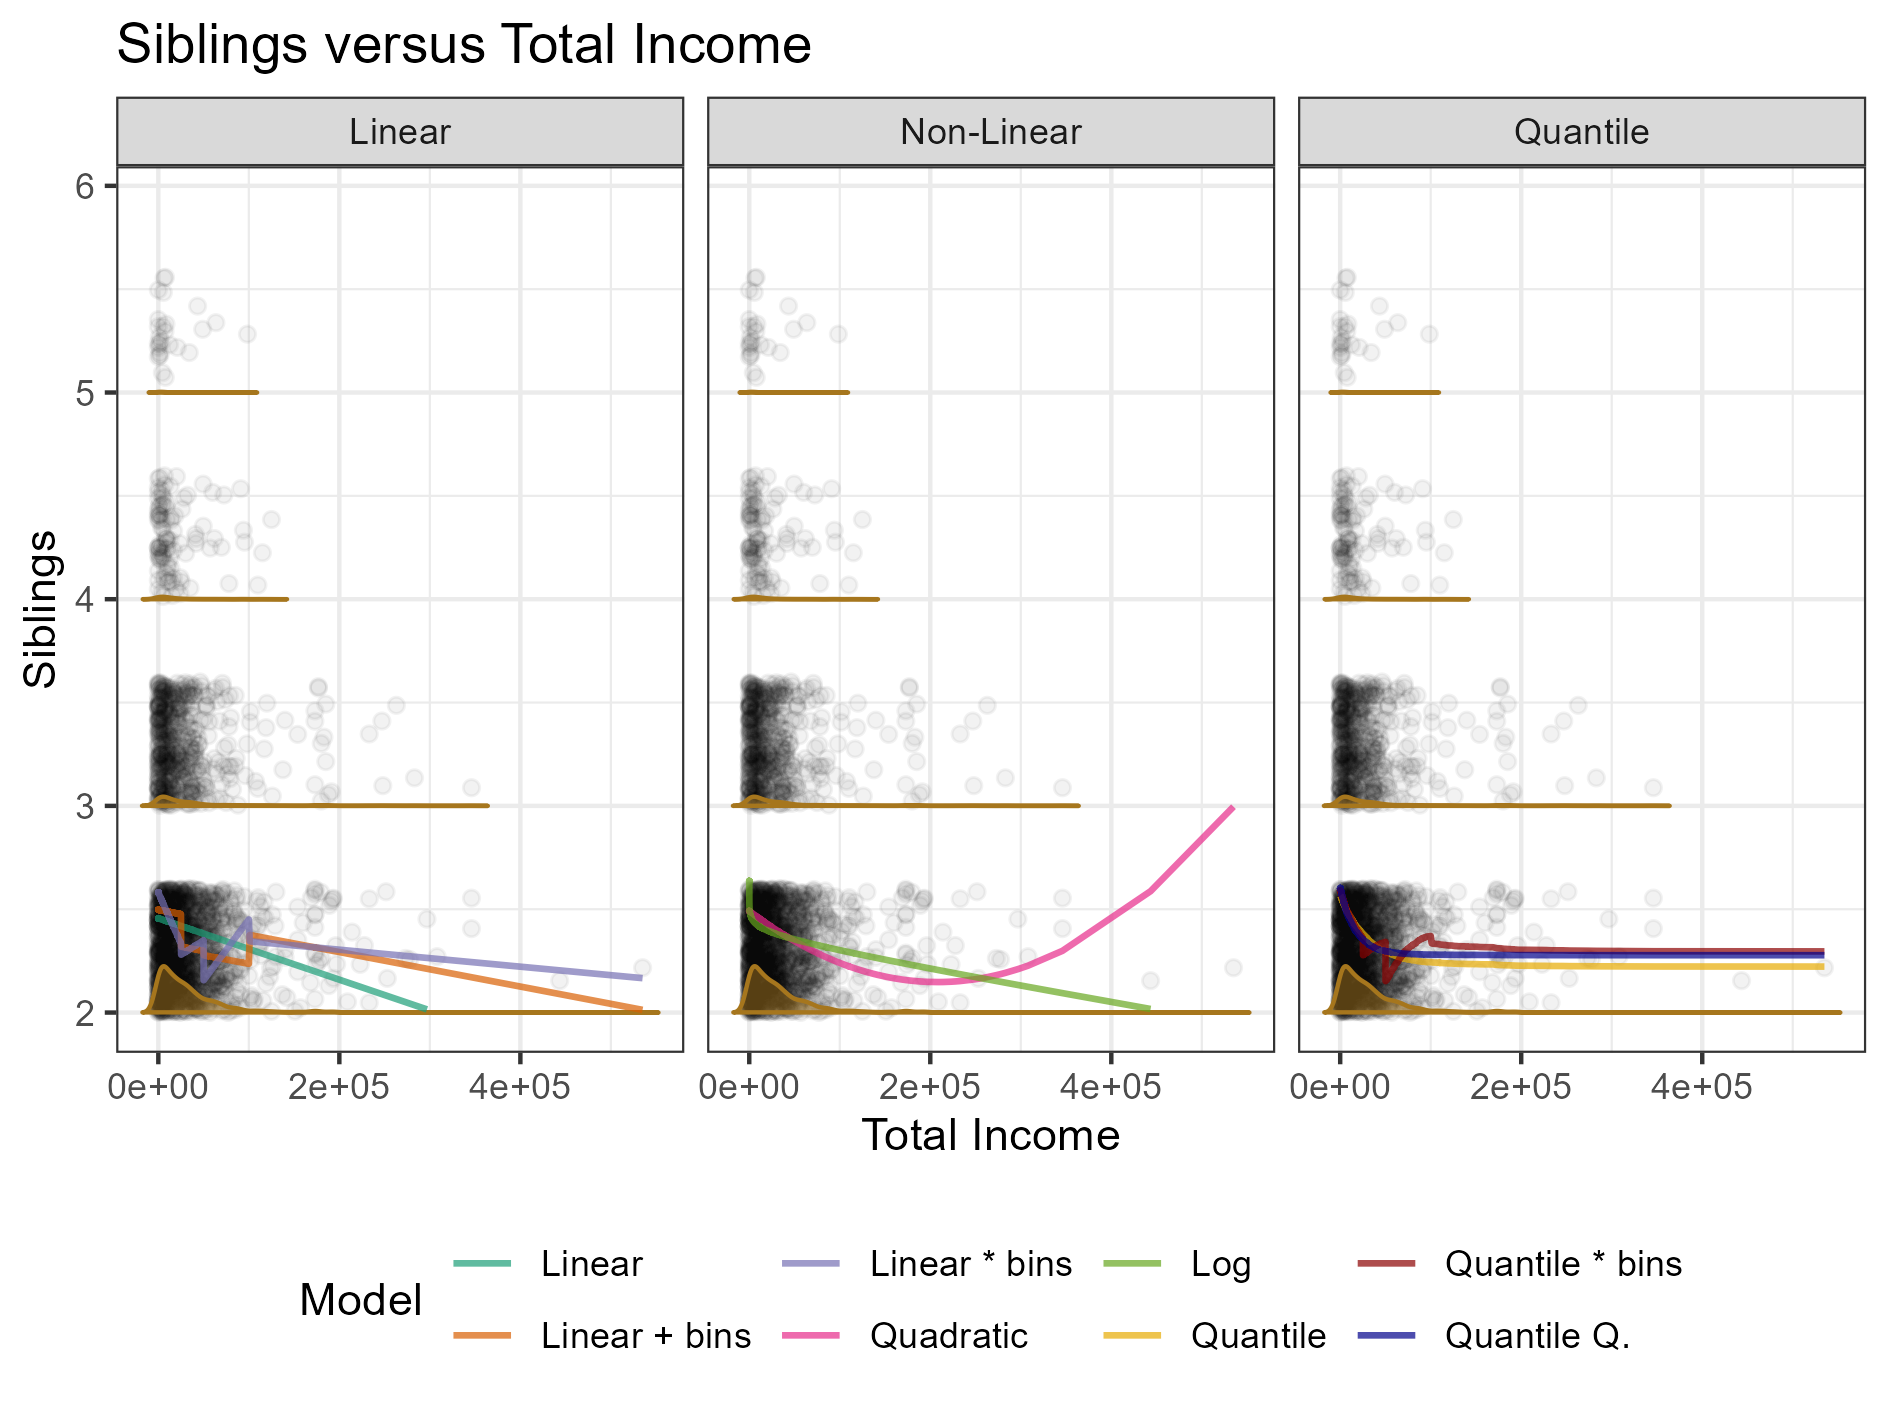
\includegraphics[width=0.9\textwidth]{Figures/cefs.png}
    \label{fig:cefs}
\end{figure}

The linear model and quadratic have their obvious limitations, with a very strange fit for large values in the edge of the data. We can see that all of the models, except for the linear one, have some sense of large number of siblings for low income families, then a initial decrease for middle income families. The linear based and quadratic models present different opposite relations for the high income families, but the log and quantil based approaches all show a stabilization around $1.75$ children. That is, it seems that, for high income, increases in income don't relate to different number of children.


\section*{Question 3}


\section*{Question 4}


\section*{Question 5}


\section*{Question 6}

The measures of quality considered were:

\begin{itemize}
    \item Number of bedrooms in the house per child (BedroomsCapta): a measure of home quality, parents that want good development for their children will increase the size of the home as the size of the family increases.
    \item Distance from ideal schooling years (YearsEduc): in Puerto Rico, children should start schooling at the age of 5, delayed children will have a negative value, and the opposite for advanced children. See the appendix for more information.
    \item Number of enrolled students per child (StudentsCapta): another measure of education quality, households where the parents enrolled all the children in a school, its value will be $1$, and lower otherwise.
    \item Number of children working per child (WorkersCapta): a negative measure of quality, if all the children are enrolled in child labor programs, the value will be $1$, and lower otherwise.
\end{itemize}

Three different specifications were considered for the regression on number of siblings: a fully saturated model with dummies for each possible value ($1$ - $7$), a linear polinomial, and a polinomial.

The results can be seen below. The regression tables (for the most relevant measures) can be seen in the section \ref{sec:results}.

\begin{figure}
    \centering
    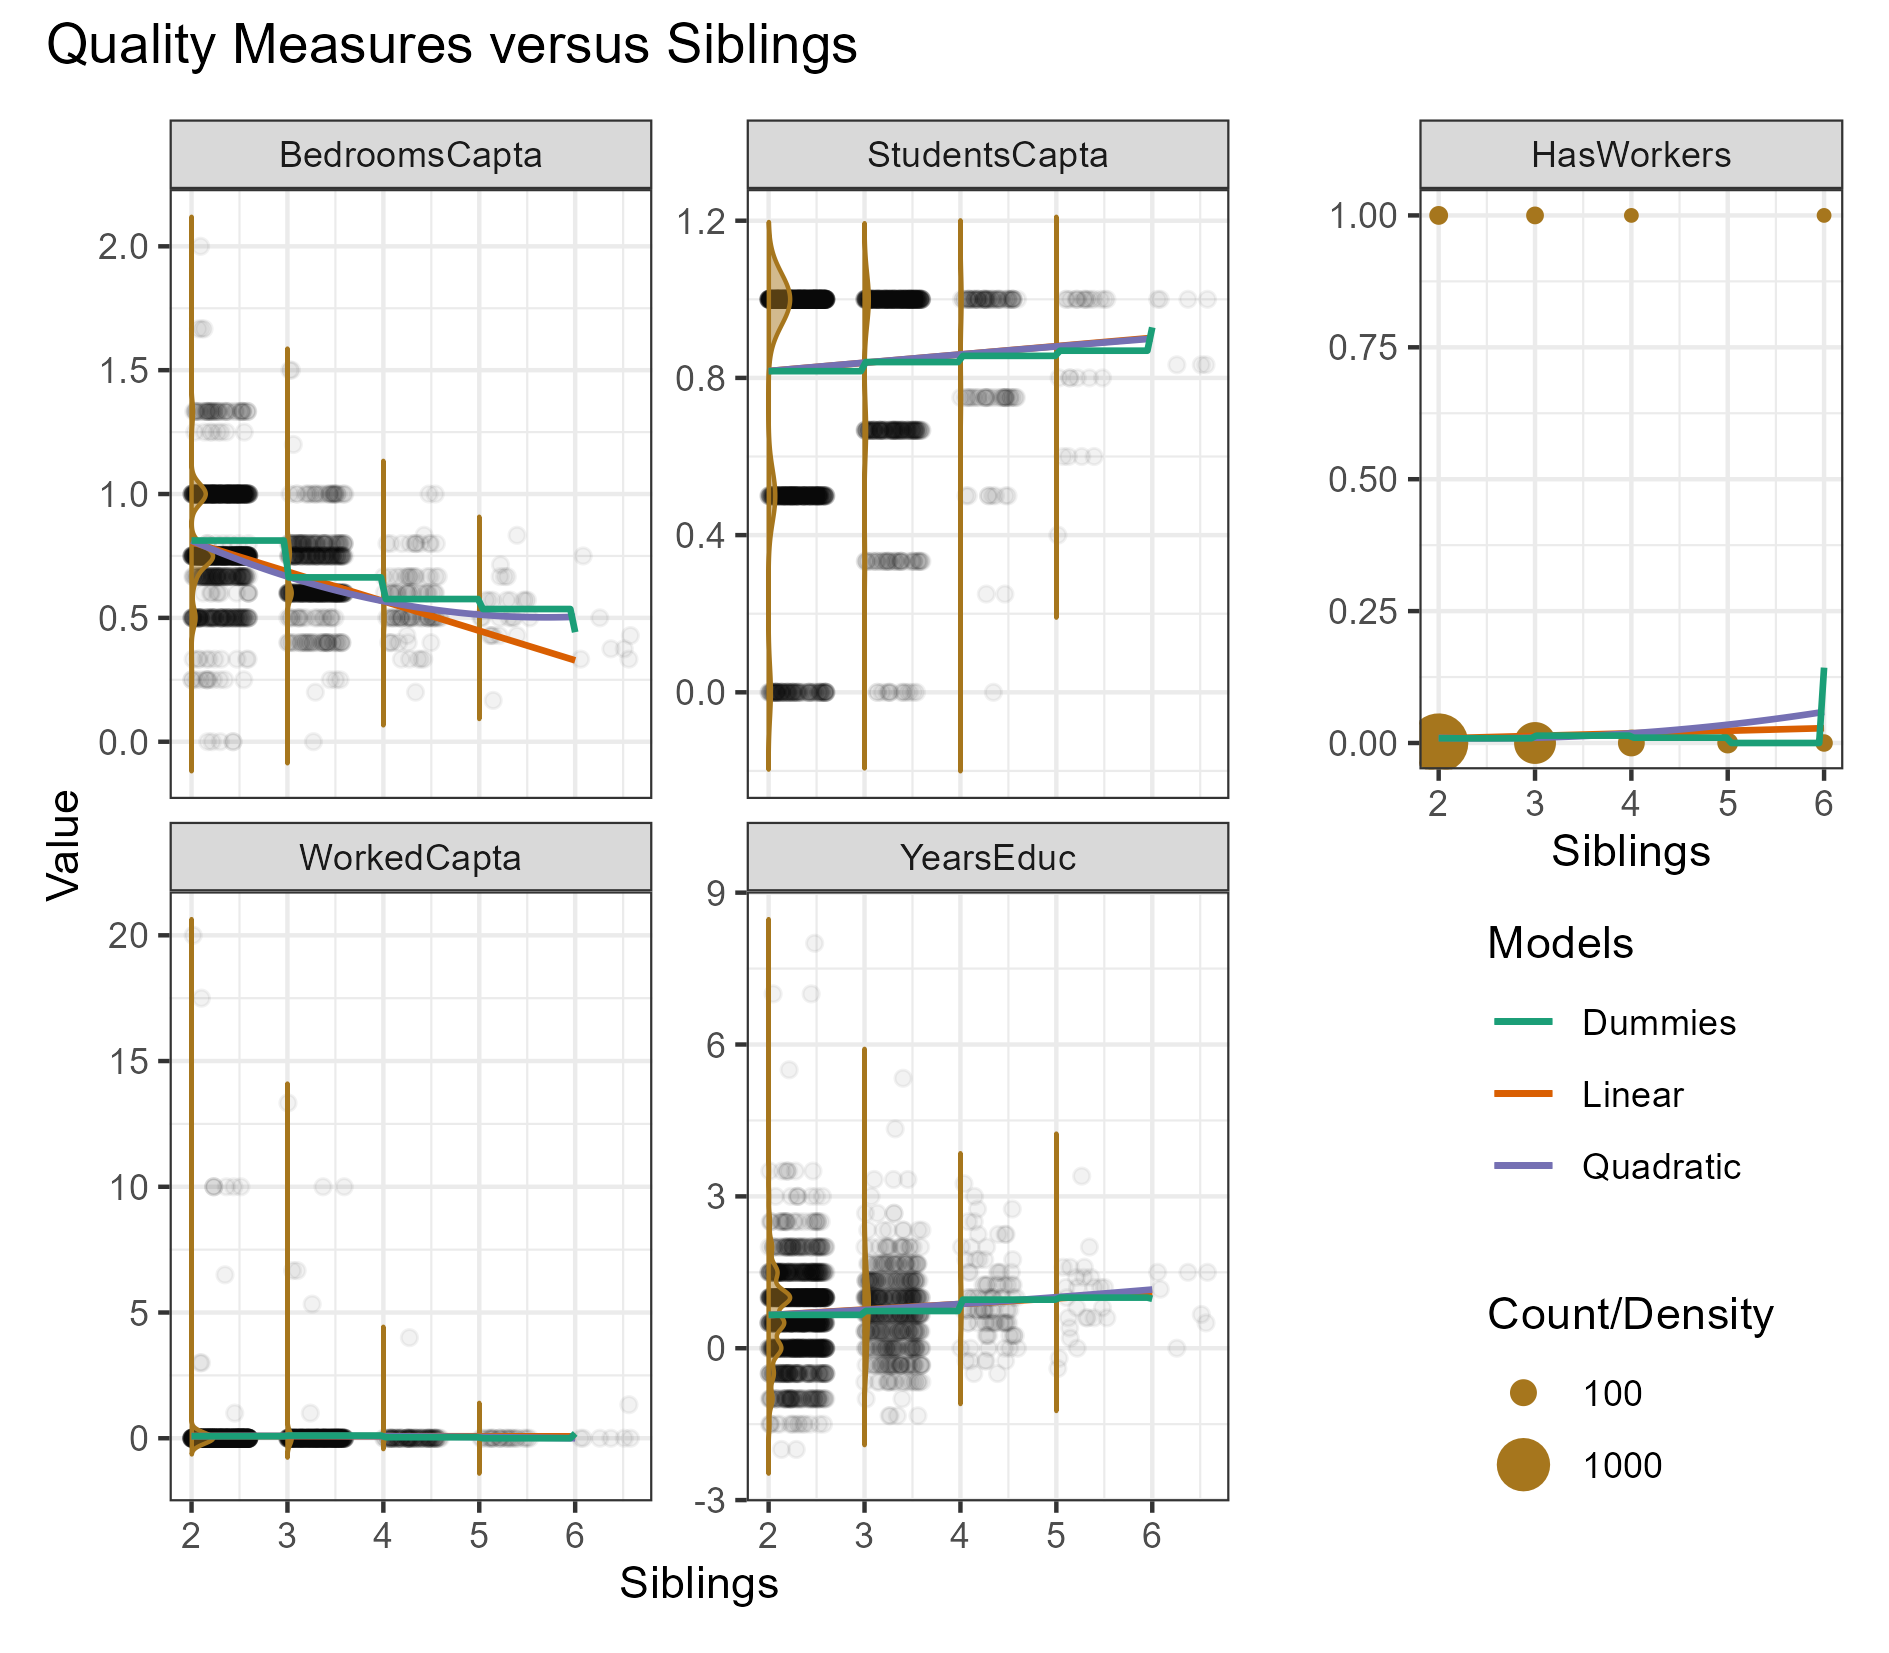
\includegraphics[width=0.9\textwidth]{Figures/quality.png}
    \label{fig:quality}
\end{figure}

First of all, we see that the quadratic polinomial matches really well the fully saturated model.

The rooms per capta presents a negative relation, as expected, but we know that part of the effect is a simple logistic problem of the rigidity of increasing the number of bedrooms in a house or changing houses, such that this is not the most interesting measure. Importantly, it might not react to unexpectedly changes in the family size. It will be kept as a probably upward (in absolute terms) biased effect.

The distance from ideal schooling years presents a very weak relation, slightly positive, the opposite of what was expected. Still, it is the best measure, and lets analise what happens when we control for confounders ahead.

The other measures aren't too interesting. The frequency of child labor is really small, and "students per capta" is a discrete measure less informative than the distance from ideal schooling years.

Not restricting the sample for certain families, such as families where the oldest son is 14 years old, can be a problem of comparability of some variables between households. At the same time, recall the discussion in the introduction about problems with sample restrictions. As the sample size is already small, the full sample was kept. In order the decrease the comparability problem, only measures that did not depend on the family ages were considered. For example, the measure "years of schooling" wouldn't be comparable, and wasn't considered.

This is not ideal, and the same worry was present in the selection of controls ahead, but the sample restriction would be too costly.


\section*{Question 7}


\section*{Question 8}
The control variables added are presented below. Each had a quick justification, normally on the style of "why does it relate to the number of siblings" and "why is it relevant for the quality measures".

\begin{itemize}
    \item Children Controls:
    \begin{itemize}
        \item Frequency of male children (MaleAvg): there is a literature on the effect of having children of a same or specific gender on the family size. Also, the gender of the children might be related to the development decision, specially the school attendance;
        \item Average children age (ChildsAgeAvg): "older families" are more probable to have already reached the planned number of children. Also,  the development decision might be different for children of different ages;
        \item Age of youngest child (ChildsAgeMin): younger children might be more present in larger families. Also, parents that have to take care of small children might focus less on the quality of the rest of the household;
        \item Presence of disabled children (HasDisabled): families that had a disabled child might have a different plan for family size. Also disabilities pose some chalenges in school attendance;
    \end{itemize}
    \item Family Controls:
    \begin{itemize}
        \item Non-atomic family size (FamSize): the number of non parents nor children in the household. Other adults might affect both the family size plan and the development decision;
        \item Income quantile (IncTotQuant): as was seen, the income of the household is one of the most important controls. The quantile version was chosen for its good fit and intuition, as presented in question 2;
        \item Percentage of welfare income (IncWel): the percentage of the family income that comes from welfare programs. It helps to better capture the effects of income, specially the different effects for the poorer families;
        \item Percentage of pension income (IncPen): the percentage of the family income that comes from pension. Important for a similar reason as above;
    \end{itemize}
    \item Parents Controls:
    \begin{itemize}
        \item Some characteristics of the parents affect the ability, interest, and time that they have available to grow big families and induce a good development for the children, such as average parents age (ParentsAgeAvg), average parents education (ParentsEducAvg), and average parents work hours (ParentsWorkAvg). The average was used as not always the father is present.
        \item It is also important to control for the cultural and social context of the family, such as parents' race (ParentsRace) and parents' citizenship (ParentsCitizenship). Both are the race/citizenship status if both parents present the same, or a value for biracial/bi-citizenship relation.
        \item Lastly, we include a control for families where at least one of the parents are step-parents (HasStep). Step parents might give a different importance to family size and development quality.
    \end{itemize}
\end{itemize}

A last relevant variable is the presence of the father in the household, as it was discussed in the introduction. But, including it would be a problem, as it can be that increases in the number of siblings causes the father to become absent, such that it might be a bad control. We can simply not control for it, and the effect for family size found will also have the effect of increasing the chance of an absent father. One would imagine that both of them work in the same direction.

The results can be seen below. There is also the visualization of the plot for the partial regression in schooling.


\begin{table}[!htbp] \centering 
  \caption{Siblings Effect - with Controls} 
  \label{} 
\begin{tabular}{@{\extracolsep{5pt}}lcccc} 
\\[-1.8ex]\hline 
\hline \\[-1.8ex] 
 & \multicolumn{4}{c}{\textit{Dependent variable:}} \\ 
\cline{2-5} 
\\[-1.8ex] & BedroomsCapta & YearsEduc & BedroomsCapta & YearsEduc \\ 
\\[-1.8ex] & (1) & (2) & (3) & (4)\\ 
\hline \\[-1.8ex] 
 Siblings & $-$0.128$^{***}$ & 0.023 &  &  \\ 
  & (7e-03) & (0.027) &  &  \\ 
  as.factor(Siblings)3 &  &  & $-$0.15$^{***}$ & 0.021 \\ 
  &  &  & (0.01) & (0.039) \\ 
  as.factor(Siblings)4 &  &  & $-$0.275$^{***}$ & 0.055 \\ 
  &  &  & (0.02) & (0.077) \\ 
  as.factor(Siblings)5 &  &  & $-$0.318$^{***}$ & 0.069 \\ 
  &  &  & (0.036) & (0.14) \\ 
  as.factor(Siblings)6 &  &  & $-$0.359$^{***}$ & 0.054 \\ 
  &  &  & (0.068) & (0.262) \\ 
 \hline \\[-1.8ex] 
Observations & 1,973 & 1,973 & 1,973 & 1,973 \\ 
R$^{2}$ & 0.291 & 0.421 & 0.297 & 0.421 \\ 
Adjusted R$^{2}$ & 0.282 & 0.414 & 0.287 & 0.413 \\ 
Residual Std. Error & 0.176 & 0.676 & 0.176 & 0.677 \\ 
\hline 
\hline \\[-1.8ex] 
\end{tabular} 
\end{table} 


\begin{figure}
    \centering
    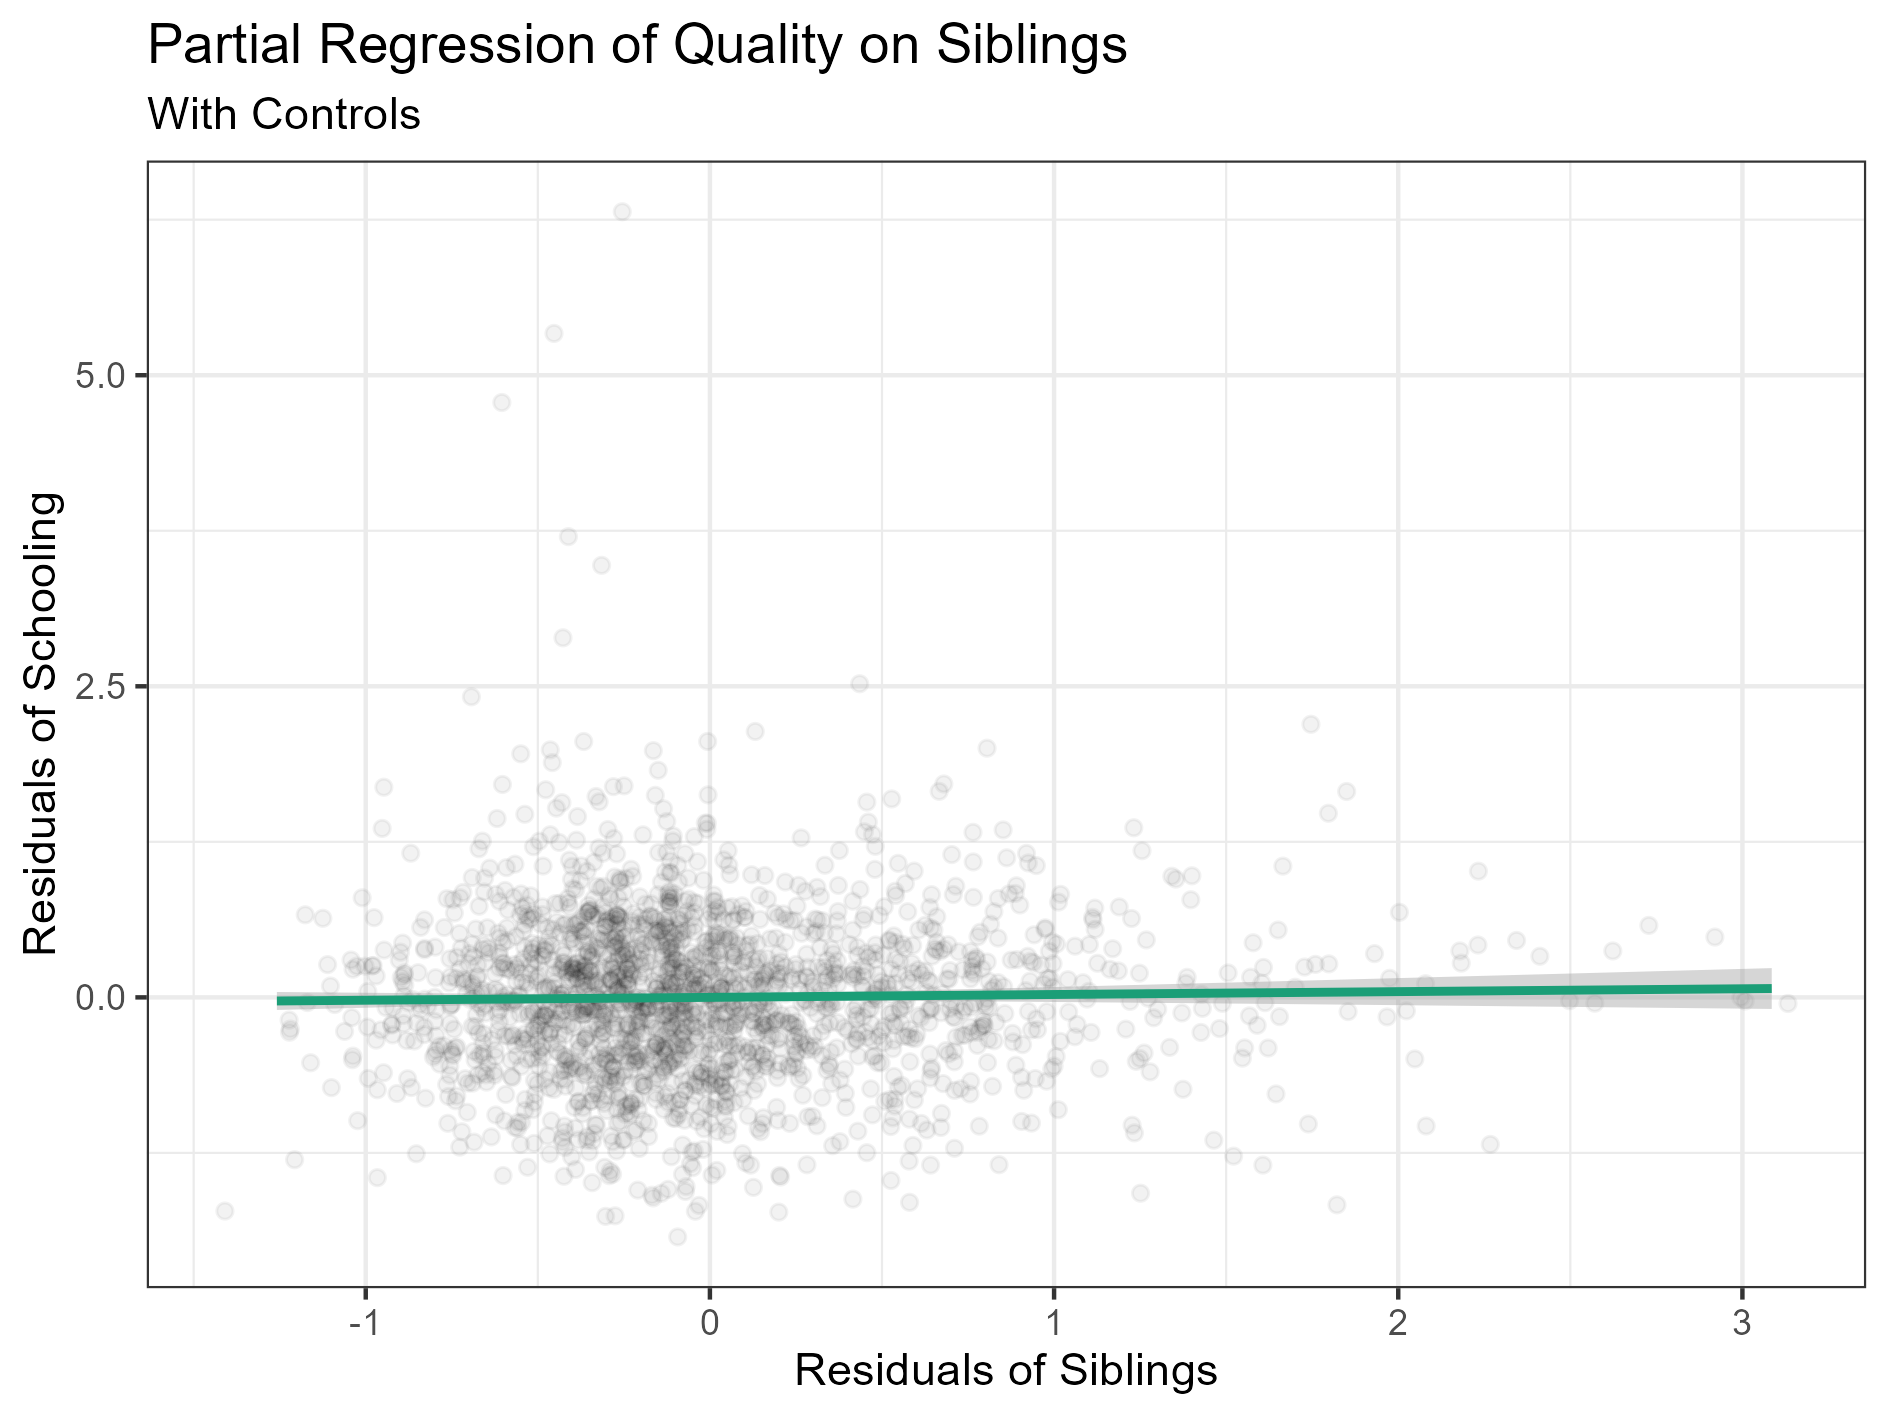
\includegraphics[width=0.9\textwidth]{Figures/quality_controls.png}
    \label{fig:quality_controls}
\end{figure}

The probably upward biased effect on "bedrooms per capta" are all negative and significant, with a stronger effect for larger families. For Years educ, the result is statistically insignificant. This goes against the existing evidence from the literature, but is understandable given the low sample size and other problems commented in the introduction.


\section*{Question 9}


\section*{Question 10}
There were a few instruments options considered:

\begin{itemize}
    \item Presence of twins as last two childrend: 
\end{itemize}

\section*{Appendix - Regression Results}\label{sec:results}


\begin{table}[H] \centering 
  \caption{Linear CEFs} 
  \label{} 
\begin{tabular}{@{\extracolsep{5pt}}lccc} 
\\[-1.8ex]\hline 
\hline \\[-1.8ex] 
 & \multicolumn{3}{c}{\textit{Dependent variable:}} \\ 
\cline{2-4} 
\\[-1.8ex] & \multicolumn{3}{c}{Siblings} \\ 
\\[-1.8ex] & (1) & (2) & (3)\\ 
\hline \\[-1.8ex] 
 IncTot & $-$0e+00$^{***}$ & $-$0e+00 & $-$1e-05$^{***}$ \\ 
  & (0e+00) & (0e+00) & (0e+00) \\ 
  IncTotCut2 &  & $-$0.157$^{***}$ & $-$0.371$^{**}$ \\ 
  &  & (0.043) & (0.17) \\ 
  IncTotCut3 &  & $-$0.178$^{***}$ & $-$0.72$^{***}$ \\ 
  &  & (0.066) & (0.232) \\ 
  IncTotCut4 &  & $-$0.037 & $-$0.194 \\ 
  &  & (0.148) & (0.169) \\ 
  IncTot:IncTotCut2 &  &  & 1e-05$^{**}$ \\ 
  &  &  & (1e-05) \\ 
  IncTot:IncTotCut3 &  &  & 2e-05$^{***}$ \\ 
  &  &  & (0e+00) \\ 
  IncTot:IncTotCut4 &  &  & 1e-05$^{***}$ \\ 
  &  &  & (0e+00) \\ 
  Constant & 2.456$^{***}$ & 2.497$^{***}$ & 2.58$^{***}$ \\ 
  & (0.019) & (0.021) & (0.031) \\ 
 \hline \\[-1.8ex] 
Observations & 1,973 & 1,973 & 1,973 \\ 
R$^{2}$ & 9e-03 & 0.021 & 0.029 \\ 
Adjusted R$^{2}$ & 9e-03 & 0.019 & 0.026 \\ 
Residual Std. Error & 0.678 & 0.675 & 0.672 \\ 
F Statistic & 18.474$^{***}$ & 10.438$^{***}$ & 8.425$^{***}$ \\ 
\hline 
\hline \\[-1.8ex] 
\end{tabular} 
\end{table} 


\begin{table}[!htbp] \centering 
  \caption{Non-linear CEFs} 
  \label{} 
\begin{tabular}{@{\extracolsep{5pt}}lcc} 
\\[-1.8ex]\hline 
\hline \\[-1.8ex] 
 & \multicolumn{2}{c}{\textit{Dependent variable:}} \\ 
\cline{2-3} 
\\[-1.8ex] & \multicolumn{2}{c}{Siblings} \\ 
\\[-1.8ex] & (1) & (2)\\ 
\hline \\[-1.8ex] 
 IncTot & $-$0e+00$^{***}$ & 0e+00 \\ 
  & (0e+00) & (0e+00) \\ 
  I(IncTot$\hat{\mkern6mu}$2) & 0e+00$^{***}$ &  \\ 
  & (0e+00) &  \\ 
  IncTotLog &  & $-$0.084$^{***}$ \\ 
  &  & (0.014) \\ 
  Constant & 1.983$^{***}$ & 2.218$^{***}$ \\ 
  & (0.022) & (0.053) \\ 
 \hline \\[-1.8ex] 
Observations & 3,328 & 3,328 \\ 
R$^{2}$ & 0.011 & 0.013 \\ 
Adjusted R$^{2}$ & 0.01 & 0.012 \\ 
Residual Std. Error & 0.867 & 0.866 \\ 
\hline 
\hline \\[-1.8ex] 
\end{tabular} 
\end{table} 


\begin{table}[!htbp] \centering 
  \caption{Quantile CEFs} 
  \label{} 
\begin{tabular}{@{\extracolsep{5pt}}lccc} 
\\[-1.8ex]\hline 
\hline \\[-1.8ex] 
 & \multicolumn{3}{c}{\textit{Dependent variable:}} \\ 
\cline{2-4} 
\\[-1.8ex] & \multicolumn{3}{c}{Siblings} \\ 
\\[-1.8ex] & (1) & (2) & (3)\\ 
\hline \\[-1.8ex] 
 IncTotQuant & $-$0.397$^{***}$ & $-$0.852$^{***}$ & $-$1.461$^{***}$ \\ 
  & (0.053) & (0.131) & (0.223) \\ 
  IncTotCut2 &  & $-$0.407 &  \\ 
  &  & (0.281) &  \\ 
  IncTotCut3 &  & $-$0.899 &  \\ 
  &  & (0.854) &  \\ 
  IncTotCut4 &  & $-$4.253 &  \\ 
  &  & (4.33) &  \\ 
  IncTotQuant:IncTotCut2 &  & 0.799$^{*}$ &  \\ 
  &  & (0.426) &  \\ 
  IncTotQuant:IncTotCut3 &  & 1.373 &  \\ 
  &  & (0.978) &  \\ 
  IncTotQuant:IncTotCut4 &  & 4.908 &  \\ 
  &  & (4.443) &  \\ 
  I(IncTotQuant$\hat{\mkern6mu}$2) &  &  & 1.044$^{***}$ \\ 
  &  &  & (0.212) \\ 
  Constant & 2.088$^{***}$ & 2.212$^{***}$ & 2.275$^{***}$ \\ 
  & (0.03) & (0.042) & (0.049) \\ 
 \hline \\[-1.8ex] 
Observations & 3,328 & 3,328 & 3,328 \\ 
R$^{2}$ & 0.017 & 0.025 & 0.024 \\ 
Adjusted R$^{2}$ & 0.016 & 0.023 & 0.023 \\ 
Residual Std. Error & 0.864 & 0.861 & 0.861 \\ 
\hline 
\hline \\[-1.8ex] 
\end{tabular} 
\end{table} 



\begin{table}[!htbp] \centering 
  \caption{Siblings Effect - no Controls} 
  \label{} 
\begin{tabular}{@{\extracolsep{5pt}}lcccc} 
\\[-1.8ex]\hline 
\hline \\[-1.8ex] 
 & \multicolumn{4}{c}{\textit{Dependent variable:}} \\ 
\cline{2-5} 
\\[-1.8ex] & BedroomsCapta & YearsEduc & BedroomsCapta & YearsEduc \\ 
\\[-1.8ex] & (1) & (2) & (3) & (4)\\ 
\hline \\[-1.8ex] 
 Siblings & $-$0.168$^{***}$ & 0.083$^{***}$ &  &  \\ 
  & (5e-03) & (0.021) &  &  \\ 
  as.factor(Siblings)2 &  &  & $-$0.227$^{***}$ & 0.028 \\ 
  &  &  & (0.01) & (0.041) \\ 
  as.factor(Siblings)3 &  &  & $-$0.373$^{***}$ & 0.111$^{**}$ \\ 
  &  &  & (0.013) & (0.055) \\ 
  as.factor(Siblings)4 &  &  & $-$0.462$^{***}$ & 0.38$^{***}$ \\ 
  &  &  & (0.025) & (0.105) \\ 
  as.factor(Siblings)5 &  &  & $-$0.509$^{***}$ & 0.48$^{**}$ \\ 
  &  &  & (0.048) & (0.202) \\ 
  as.factor(Siblings)6 &  &  & $-$0.591$^{***}$ & 0.342 \\ 
  &  &  & (0.096) & (0.4) \\ 
  Constant & 1.173$^{***}$ & 0.524$^{***}$ & 1.033$^{***}$ & 0.634$^{***}$ \\ 
  & (0.011) & (0.044) & (7e-03) & (0.03) \\ 
 \hline \\[-1.8ex] 
Observations & 3,328 & 3,328 & 3,328 & 3,328 \\ 
R$^{2}$ & 0.247 & 5e-03 & 0.262 & 6e-03 \\ 
Adjusted R$^{2}$ & 0.247 & 4e-03 & 0.261 & 5e-03 \\ 
Residual Std. Error & 0.256 & 1.056 & 0.253 & 1.056 \\ 
\hline 
\hline \\[-1.8ex] 
\end{tabular} 
\end{table} 


%
\begin{table}[!htbp] \centering 
  \caption{Siblings Effect - with Controls} 
  \label{} 
\begin{tabular}{@{\extracolsep{5pt}}lcccc} 
\\[-1.8ex]\hline 
\hline \\[-1.8ex] 
 & \multicolumn{4}{c}{\textit{Dependent variable:}} \\ 
\cline{2-5} 
\\[-1.8ex] & BedroomsCapta & YearsEduc & BedroomsCapta & YearsEduc \\ 
\\[-1.8ex] & (1) & (2) & (3) & (4)\\ 
\hline \\[-1.8ex] 
 Siblings & $-$0.128$^{***}$ & 0.023 &  &  \\ 
  & (7e-03) & (0.027) &  &  \\ 
  as.factor(Siblings)3 &  &  & $-$0.15$^{***}$ & 0.021 \\ 
  &  &  & (0.01) & (0.039) \\ 
  as.factor(Siblings)4 &  &  & $-$0.275$^{***}$ & 0.055 \\ 
  &  &  & (0.02) & (0.077) \\ 
  as.factor(Siblings)5 &  &  & $-$0.318$^{***}$ & 0.069 \\ 
  &  &  & (0.036) & (0.14) \\ 
  as.factor(Siblings)6 &  &  & $-$0.359$^{***}$ & 0.054 \\ 
  &  &  & (0.068) & (0.262) \\ 
 \hline \\[-1.8ex] 
Observations & 1,973 & 1,973 & 1,973 & 1,973 \\ 
R$^{2}$ & 0.291 & 0.421 & 0.297 & 0.421 \\ 
Adjusted R$^{2}$ & 0.282 & 0.414 & 0.287 & 0.413 \\ 
Residual Std. Error & 0.176 & 0.676 & 0.176 & 0.677 \\ 
\hline 
\hline \\[-1.8ex] 
\end{tabular} 
\end{table} 



\section*{Appendix - Exploratory Analisys}\label{sec:explore}


%\section*{References}
%\bibliography{bibliography.bib}
%\bibliographystyle{plain}

\end{document}